\chapter{IOSharp}\label{C:IOSharp development}

In this chapter it will be explained how was defined and architected, designed and implemented the core of IOSharp disaggregating the different parts and explaining each one.
\\
\\
First of all it will be explained the project design explaining which two options where at project definition, then the implementation is explained for the different IO ports and communication standards used in this project. Finally, it will be explained how is done the port mapping to work between different boards and devices.

\section{Planning the development}\label{S:Design}
At project start, the development was focused on a tiny Linux board called RaspberryPi. This device was designed by RaspberryPi Foundation in England taking in mind the kids around the world and helping them to provide cheap tools to be introduced in computer science. It is an interesting board for its features, offering basic IO using the provided GPIOs, it also provides a SPI module for peripheral communication, an I$^{2}$C and UART interface also for transmissions between external components and the device itself.
\\
In addition to the interfaces mentioned above, it also has some desktop interesting features like USB ports which practically can accept any device that works on Linux for instance a WiFi, Bluetooth, ZigBee or any stick for wireless transmissions, HDMI for graphics and user interface and Ethernet for network communications. Apart from this IO characteristics, it also mounts a decent ARMv6 (CPU) running at 700MHz on stock frequency and being overclocked to 1GHz without problems. Together with the CPU 512MB of RAM are provided which is enough for normal desktop usage (surfing, emailing and office) and for embedded projects.
\\
\\
After choosing the target device, two implementing options where designed and analysed. Each one has its own benefits and problems that are going to be explained in the following sections. As an introduction to the options that were considered where the use of the specific tools and libraries for the RaspberryPi and its CPU, this should help on achieving high efficiency when deployed on the device. On the other hand, trying to develop the project as widely as possible to give the chance of running under any Linux (or similar operating systems like Unix or Android) avoiding the exclusion of other devices.

\subsection{Focused on RaspberryPi}\label{SS:}
\subsection{Focused on Linux in General}\label{SS:}
Since the design of IOSharp was focused on reach any device capable of execute C\# and not only the RasperryPi the best solution could be use 

\section{Implementation}\label{S:Implementation}
Remember that as it was explained on the introduction, the goal of this thesis is deploy and run successfully the HomeSense platform on a RaspberryPi. Taking in mind this, some modules where required to develop in order to accomplish with this requirement. In this case the GPIO, Interrupts, SPI and UART need to work in order to use the different components of HomeSense.

\subsection{GPIO}\label{SS:GPIO}
In order to implement the GPIO ports in NETMF it will be used the IOPorts.cs file which contain the structure for Input, Output, Tristate and Interrupt ports, the first three will be explained in this section whereas the interrupt port will have a dedicated one.
\\
Below is explained the different options on implementing GPIOs in Linux, which has been chosen and how has been implemented in this project.

\subsubsection{Implementation Options}\label{SSS:Implementation-Options}
GPIO acronym stands for General Purpose Input Output which are Ports on systems that are capable of generating an output or reading an input. Normally embedded systems work with ports at 3.3V, other devices had low power supply like 2V. And it is not strange that many of them are tolerant to 5V in input.
\\
In case of the Netduino and RaspberryPi the ports on both devices run at 3.3V and also the different test hardware modules used in this thesis.
\\
\\
The GPIOs in Linux can be controlled in several ways, the most common and simple is use the userspace which stands for a set of directories with readable and writeable files representing the ports of the MCU or CPU. On the other hand the Linux kernel also provides a library and a module in order to control the different pins.
\\
The decision must be done between this two systems, in order to use any of this solutions the GPIO must be activated in kernel, many desktop Linux distributions have GPIO disabled and that's why the kernel must be recompiled enabling this feature. Basically GPIOs and SYSFS must be activated on kernel configuration, after compiling and installing the new kernel both methods will be enabled.
\\
In case of Linux operating systems designated for embedded devices, for example the RaspberryPi or CubieBoard, will have the Input/Output Ports enabled by default.
\\
One of the most curious things that where found at studding this possibilities was that Android is capable to use this ports. Although it cannot seem an interesting feature nowadays android is everywhere and can run in many devices, so is another reason to try to fetch this this sector in future versions of this software.

\subsubsection{Using GPIO from SYSFS}\label{SSS:GPIO-SYSFS}
Since each solution can be used in this project and both are available in any Linux OS when the kernel is properly compiled the chosen option was control the GPIO through the SYSFS in order to simplify both the development and the testing.
\\
Use the Input/Output ports using the userspace is really simple and that one of the biggest reasons, the easiness of testing and debugging the functionality. It is easier to read or write a file in order to test if the control of the GPIOs is successful rather than debugging a C function embedded in a library.
\\
\\
As it was said before, in userspace the control of the GPIOs is carried by several files and directories located under \textit{/sys/class/gpio} directory. In this directory there are two files which are called export and unexport, the first one is used to enable a GPIO while the second one will be used to disable it. After enabling a GPIO a new folder will be created representing the enabled port, for instance if port 2 is enabled, a folder called gpio2 will be created. Inside this new folder there will be several files, the direction file describes how port should work, if the desired function is as an input port an "in" must be written in the file whereas "out" must be write for an output port. After setting the port direction the value file comes in which will do the functions of reading the port in case of input ports, or write 0 or 1 through it if the port is described as an output. To do this, just read this file to read an incoming value, or write 1 for active-high or 0 for active-low.

\subsubsection{Implementing in NETMF}\label{SSS:Implementing-GPIO-NETMF}
Taking in mind that this implementation has to be done over the existing code extracted from the \textit{IOPorts.cs} is important to design how to do it properly, in this case a \textbf{GPIOManager} has been created using a singleton pattern, in order to restrict one instantiation of this class among all the code, and simplify the use of this class.
\\
This manager will be in charge of enabling, disabling and operating the different ports. Also it will control which ports are enabled in order to avoid problems, \textcolor{red}{i.e instantiating the same port twice will make the GPIOManager throw an exception so it can prevent hardware damages.}
\\
For GPIO implementation Output, Input and Tristate ports will be required, below you can see how look the classes provided by NETMF. This classes will consume the GPIOManager explained above.

\begin{figure}[H]\begin{center}
 \centering
  \captionsetup{justification=centering}
  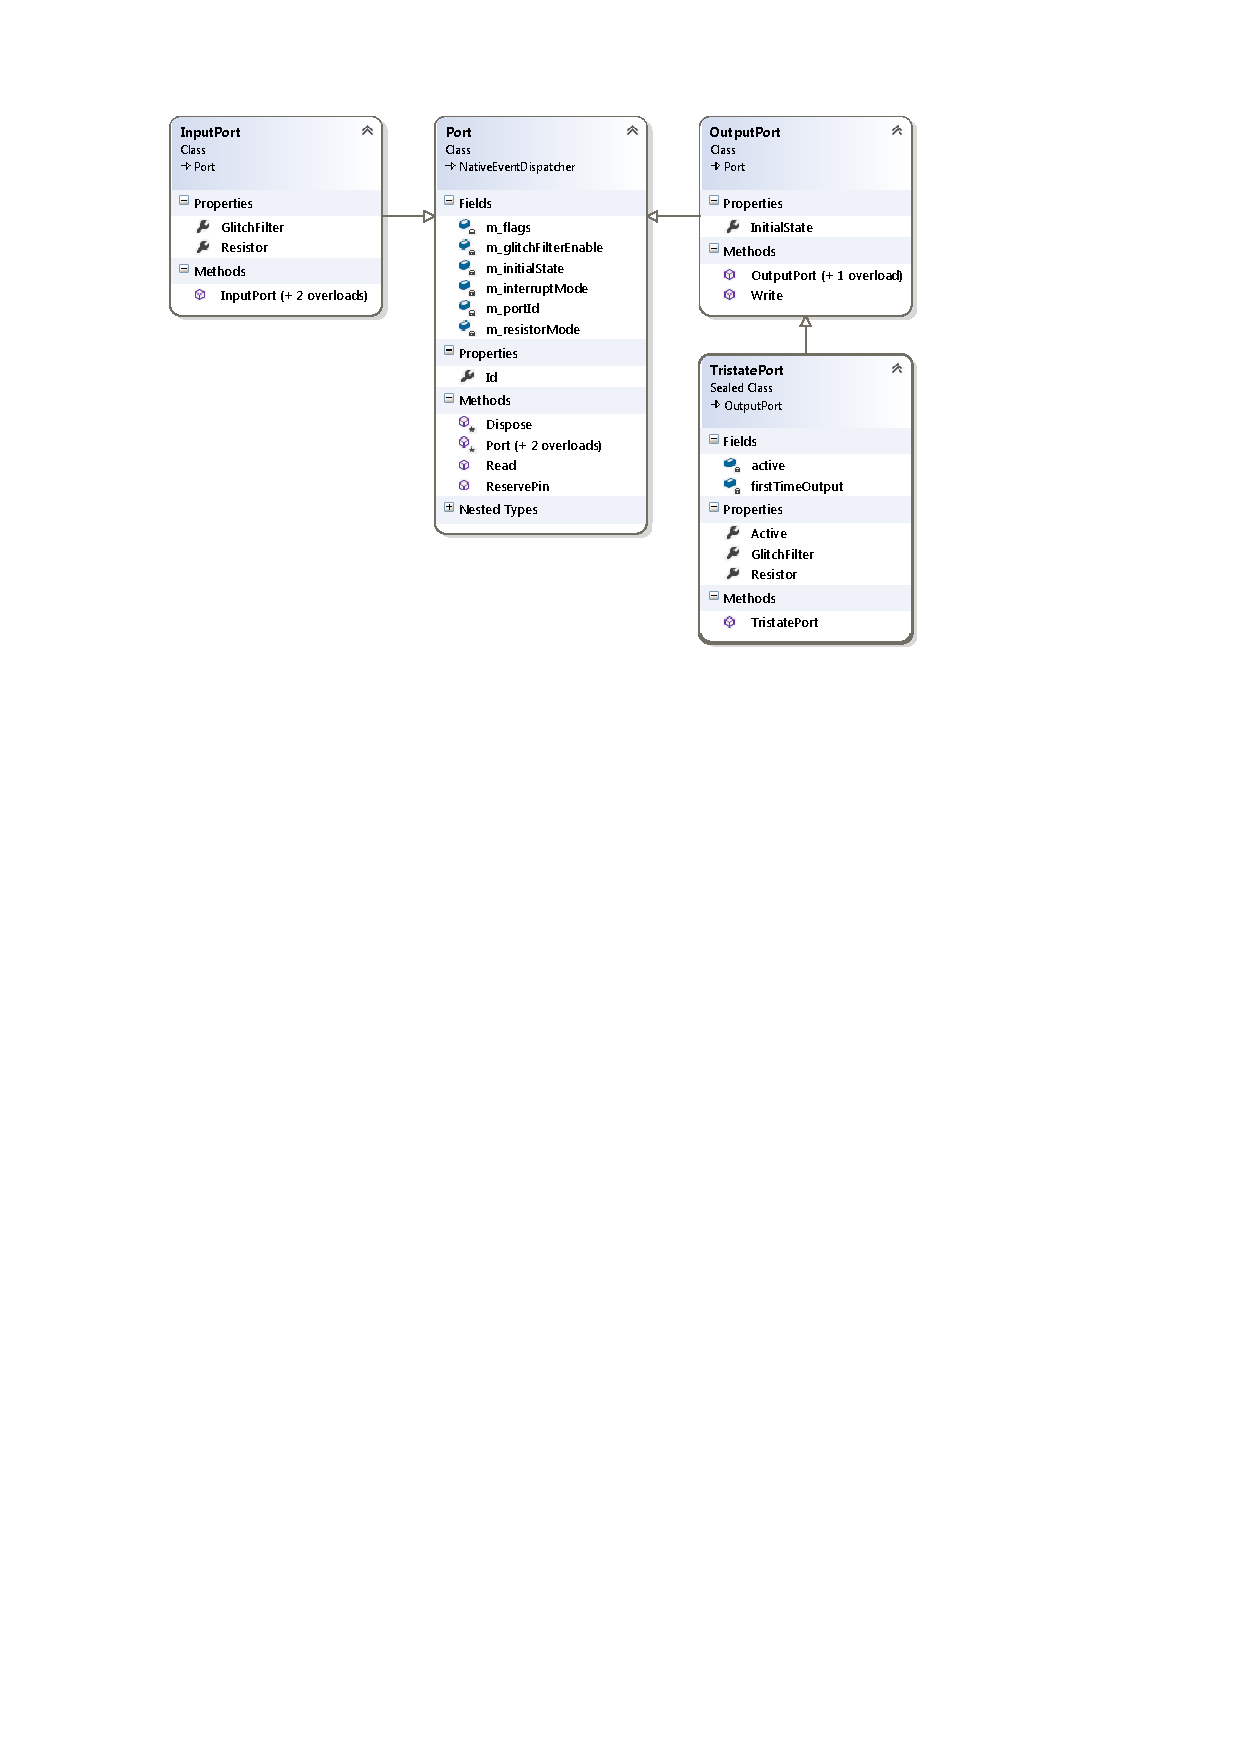
\includegraphics[width=1\textwidth]{pictures/iosharp/gpio}
  \caption{UML Diagram of NETMF Port and its inheritance \label{fig:gpio-uml}}
\end{center}\end{figure}
As is shown each Port type inherit from Port object which implements the methods to enable or disable a port (Port and Dispose methods), Read which is used to obtain the current state of the port i.e read an input value or know in which state is configured the output port. Finally it also has a ReservePin and as its name says, it is used to reserve a pin for future usage. Taking a look on the left box it can be seen the InputPort which inherits from Port. It does not have any special method and its constructor suppers to Port class. On the right side there is an OutputPort also inheriting from Port which implements a new method called Write that its used to write a state through the port, active high or active low. TristatePort also inherits from OutputPort, a NETMF TristatePort is a type of port capable of commuting between input or output port, i.e with a TristatePort is possible to control 2 leds which one of them is connected in pull-up and the other one in pull-down, so with this TristatePort is possible to light one, the other, if it is configured as an output port either on active high or low, or turning the TristatePort to an input port will avoid the lightning of any led.

\subsection{Interrupt}\label{SS:RaspberryPi-NETMF}
After implementing the GPIO and taking in mind the needs for HomeSense an interrupt system was needed for the future \gls{SPI}  code block. Although the \gls{BCM2835} supports native interruptions via \gls{IRQ} at the time of this project the RaspberryPi did not support GPIO interruptions from the Linux Kernel using the \gls{IRQ}.

\begin{figure}[H]\begin{center}
 \centering
  \captionsetup{justification=centering}
  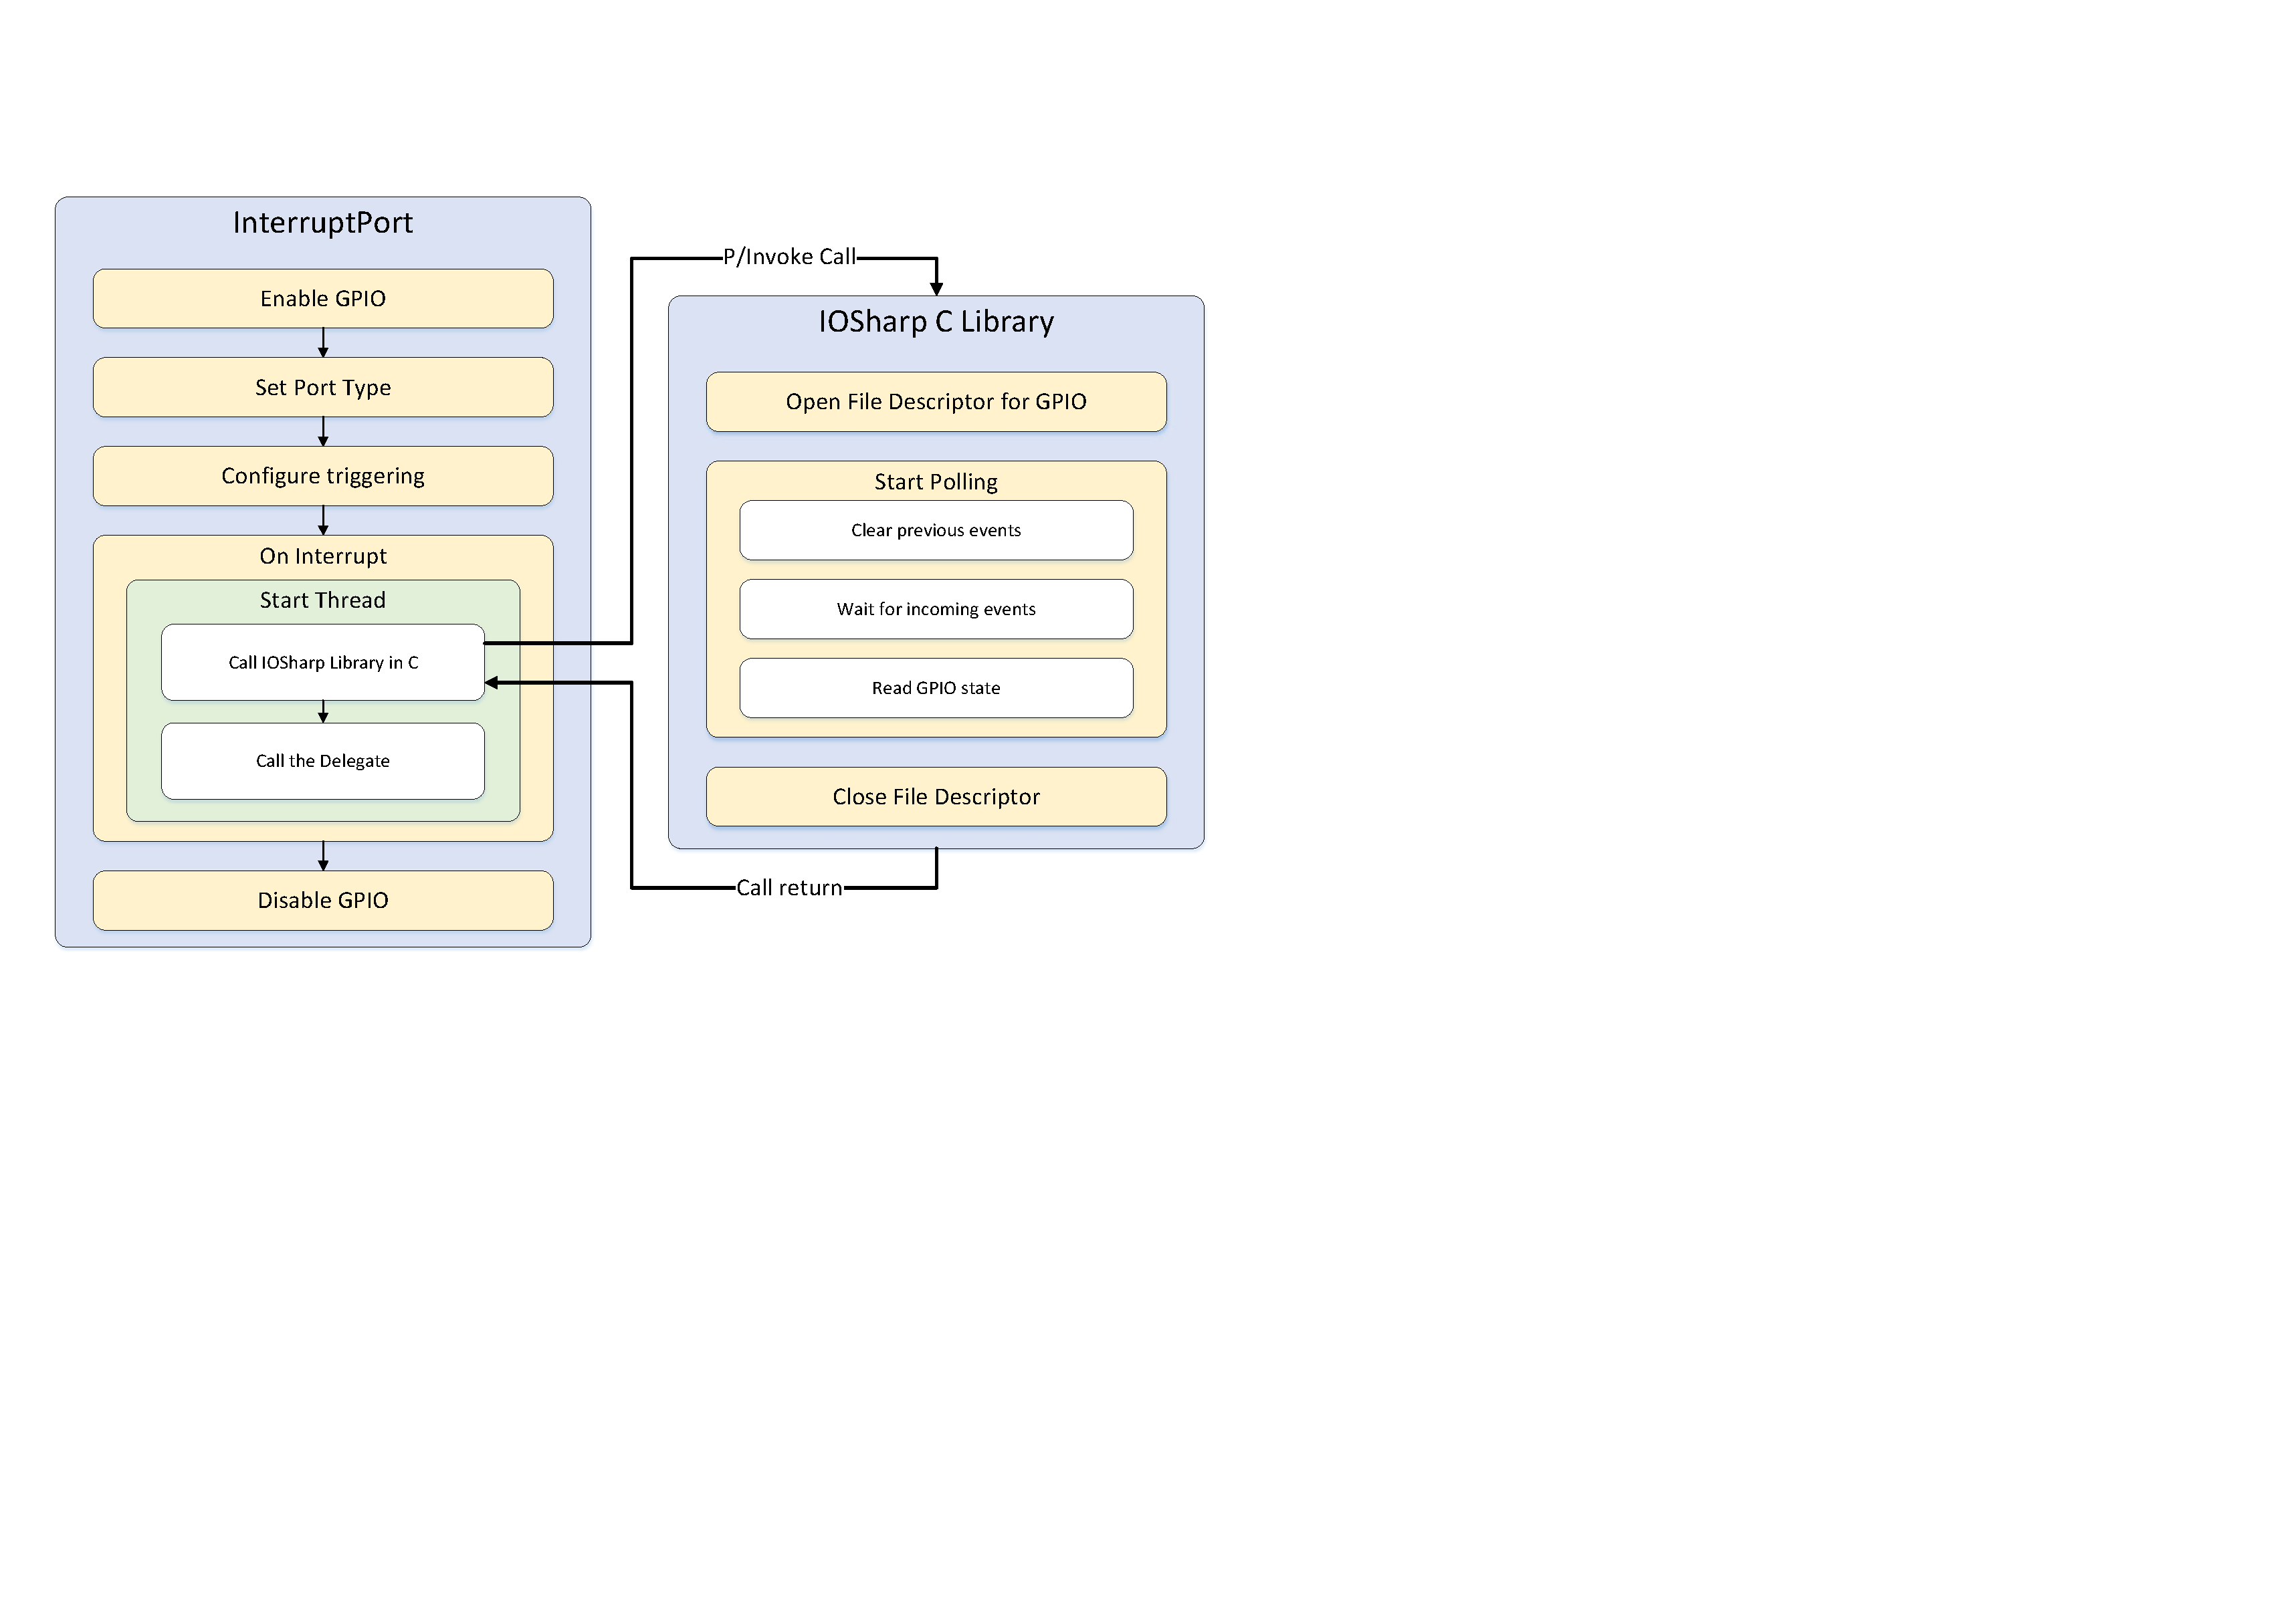
\includegraphics[width=1\textwidth]{pictures/iosharp/interrupt-schema}
  \caption{Representation of the Interrupt Port flow \label{fig:interrupt-schema}}
\end{center}\end{figure}

\subsection{SPI}\label{SS:IOSharp-SPI}
Once the port interruptions where working it was possible to start designing and implementing the SPI code block for IOSharp.
\subsection{UART}\label{SS:IOSharp-UART}


\section{Port Mapping}\label{S:Port-Mapping}
\subsection{HardwareProvider}\label{SS:HardwareProvider}



